\documentclass[12pt]{beamer}
\usetheme{default}
\usefonttheme{serif}

\usepackage{attrib}

\usepackage[backend=biber, citestyle=authoryear]{biblatex}
\addbibresource{references.bib}

\usepackage{tikz}
\usetikzlibrary{arrows,automata}

\usepackage{minted}

\usepackage{graphicx}

\usepackage{tabularx}
\usepackage{colortbl}

\usepackage{wasysym}

\author{Michael Walker}
\title{Runtime Verification}
\institute{Department of Computer Science\\
  University of York\\
  \texttt{msw504@york.ac.uk}
}

\begin{document}

\begin{frame}[plain]
  \titlepage
\end{frame}

%%%%% 1 Minute (1)

\begin{frame}{Outline}
  \tableofcontents

  \begin{center}
    See the handout for literature references.
  \end{center}
\end{frame}

%%%%% 5 Minutes (6)

\section{Static Analysis is Hard}
\label{sec:statann}

\begin{frame}{Static Analysis}
  \textbf{Static Analysis:} The (fully or partially) automatic process
  of proving properties of programs prior to executing them.

  \visible<2->{
    \begin{itemize}
      \item Type checking
      \item Memory safety
      \item Deadlock/livelock freedom
      \item Schedulability
    \end{itemize}
  }
\end{frame}

\begin{frame}{Rice's Theorem: \small A Nemesis Arises!}
  % PAPERS: rice (corollary b)

  \begin{quote}
    ``If $\mathcal P$ is any property possessed by some, but not all,
    recursively enumerable sets, then there exists no effective
    general method for deciding, given a set $\alpha$ by means of a
    partial recursive function enumerating it, whether or not $\alpha$
    has the property $\mathcal P$.  [\ldots] Of course, there will
    exist special methods for particular functions.''

    \attrib{Rice's Theorem, Corollary B, 1953}
  \end{quote}
\end{frame}

\begin{frame}{Practical Static Analysis: \small Defeating Rice}
  Rice's theorem:
  \begin{itemize}
    \item applies to Turing machines,
    \item refers to exact results,
    \item refers to a fully automatic analysis.
  \end{itemize}

  \visible<2->{
    \vspace{0.25cm}

    We can:
    \begin{itemize}
      \item use more specific systems,
      \item use approximations,
      \item introduce human contribution.
    \end{itemize}
  }

  \visible<3->{
    \vspace{0.25cm}

    Still very difficult.
  }
\end{frame}

%%%%% 15 Minutes (21)

\section{Runtime Verification}
\label{sec:runver}

\begin{frame}
  \begin{center}
    \Large Static analysis is getting harder

    \visible<2>{
      \vspace{0.25cm}
      \ldots but maybe there is another way.
    }
  \end{center}
\end{frame}

\begin{frame}{Runtime Verification}
  % NON-PAPERS: rv01

  \begin{quote}
    ``The ultimate longer term goal is to investigate whether the use of
    lightweight formal methods applied during the execution of
    programs is a viable component to the current heavyweight methods
    proving programs correct always before their execution, such as
    model checking and theorem proving.''

    \attrib{K. Havelund \& G. Rosu, RV'01}
  \end{quote}
\end{frame}

%%%%%%%%%% 7 Minutes (13)

\subsection{Design by Contract}
\label{sec:runver-dbc}

\begin{frame}{Design by Contract}
  % PAPERS: eiffel

  \begin{itemize}
    \item Introduced in 1988 in Eiffel \parencite{eiffel}.
    \item Functions have associated pre- and postconditions.
    \item Preconditions are assumed true when the function is called.
    \item Postconditions must be true if the function terminates
      and the precondition was met.
  \end{itemize}

  \visible<2->{
    \vspace{0.25cm}

    Contracts can be:

    \begin{itemize}
      \item simply assumed; or
      \item verified statically; or
      \item enforced at runtime.
    \end{itemize}
  }
\end{frame}

\begin{frame}{Design by Contract}
  \begingroup
  \renewcommand{\arraystretch}{2}
  \begin{tabularx}{\textwidth}{|X|c|c|}
    \hline
    & Learning curve & Automated reasoning\\

    \hline
    \textbf{DSL} & \cellcolor{red!25} {\Large \frownie} &
    \cellcolor{green!25} {\Large \smiley}\\

    \hline
    \textbf{Host} & \cellcolor{green!25} {\Large \smiley} &
    \cellcolor{red!25} {\Large \frownie}\\

    \hline
  \end{tabularx}
  \endgroup
\end{frame}

\subsubsection{Domain-specific Languages}
\label{sec:runver-dbc-dsl}

\begin{frame}[fragile]{Contract Languages: \small JML}
  % PAPERS: jml

  JML \parencite{jml} has

  \begin{itemize}
    \item data and loop invariants,
    \item ghost variables,
    \item method frame specification,
    \item model methods.
  \end{itemize}
\end{frame}

\begin{frame}{JML Example}
  \inputminted[fontsize=\footnotesize]{java}{jmlstack.java}
\end{frame}

\begin{frame}{Contract Languages: \small BCSL / BML}
  % PAPERS: bcsl, bml

  BCSL \parencite{bcsl} (later BML \parencite{bml})

  \begin{itemize}
    \item JML analogue for Java bytecode
    \item Can be produced from JML
    \item Developed for the possibility of proof-carrying code
    \item Compact binary representation of contracts
  \end{itemize}
\end{frame}

\begin{frame}[fragile]{BML Example}
  \begin{verbatim}
{| requires lv[2] > 0
   ensures lv[2] == \old(lv[2]) - 1
   ensures \result == \old(lv[3]) |}
  \end{verbatim}

  \vspace{0.25cm}

  Predicates: \textbf{20 bytes} (vs \textbf{80}, or \textbf{640} bits)

  \vspace{0.25cm}

  Predicates + metadata: \textbf{362 bits}.
\end{frame}

\begin{frame}[fragile]{BML Example}
  \footnotesize
  \begin{tikzpicture}[level/.style={sibling distance=6cm/#1}]
    \node (a) {\&\&}
      child {node (b) {==}
        child {node (c) {lv}
          child {node (d) {2}}
        }
        child {node (e) {-}
          child {node (f) {old}
            child {node (g) {lv}
              child {node (h) {2}}
            }
          }
          child {node (i) {int}
            child {node (j) {1}}
          }
        }
      }
      child {node (k) {==}
        child {node (l) {result}}
        child {node (m) {old}
          child {node (n) {lv}
            child {node (o) {2}}
          }
        }
      };

    \path (a) -- (b);
    \path (a) -- (k);
    \path (b) -- (c);
    \path (b) -- (e);
    \path (c) -- (d);
    \path (e) -- (f);
    \path (e) -- (i);
    \path (f) -- (g);
    \path (g) -- (h);
    \path (i) -- (j);
    \path (k) -- (l);
    \path (k) -- (m);
    \path (m) -- (n);
    \path (n) -- (o);
  \end{tikzpicture}
\end{frame}

\begin{frame}[fragile]{BML Example}
  \footnotesize
  \begin{tikzpicture}[level/.style={sibling distance=6cm/#1}]
    \node (a) {0x02}
      child {node (b) {0x08}
        child {node (c) {0x90}
          child {node (d) {0x02}}
        }
        child {node (e) {0x28}
          child {node (f) {0x99}
            child {node (g) {0x90}
              child {node (h) {0x02}}
            }
          }
          child {node (i) {0x40}
            child {node (j) {0x01}}
          }
        }
      }
      child {node (k) {0x08}
        child {node (l) {0x52}}
        child {node (m) {0x99}
          child {node (n) {0x90}
            child {node (o) {0x02}}
          }
        }
      };

    \path (a) -- (b);
    \path (a) -- (k);
    \path (b) -- (c);
    \path (b) -- (e);
    \path (c) -- (d);
    \path (e) -- (f);
    \path (e) -- (i);
    \path (f) -- (g);
    \path (g) -- (h);
    \path (i) -- (j);
    \path (k) -- (l);
    \path (k) -- (m);
    \path (m) -- (n);
    \path (n) -- (o);
  \end{tikzpicture}
\end{frame}

\begin{frame}{Contract Languages}
  \begin{itemize}
    \item JML: Has a Java-like syntax written in special comments,
      allows actual Java to define model methods.

    \item BCSL \& BML: Use Java class attributes to store encoded
      contracts in a binary format.
  \end{itemize}

  Static proof tools exist for both, runtime instrumentation and
  monitoring exists for JML.
\end{frame}

\subsubsection{Re-using the Host Language}
\label{sec:runver-sbc-aop}

\begin{frame}{Design by Contract: \small Piggy-backing on the host language}
  % PAPERS: jcontractor, ezcontract

  \only<1>{
    \begin{itemize}
      \item Rather than define a new contract language, re-use the host
        language.

      \item May define high-level functions approximating a DSL.

      \item Easy to use for runtime monitors.

      \item Difficult to use for static analysis.
    \end{itemize}
  }

  \only<2>{
    jContractor \parencite{jcontractor} specifies contracts for
    methods in separate methods following a naming scheme:

    \begin{description}
      \item[Original:]     \texttt{T foo($\ldots$)}
      \item[Precondition]  \texttt{boolean foo\_Precondition($\ldots$)}
      \item[Postcondition] \texttt{boolean foo\_Postcondition($\ldots$, T RESULT)}
    \end{description}

    Implements checking by on-the-fly bytecode manipulation.

    \begin{itemize}
      \item Overhead is only incurred if the code is run with
        jContractor.

      \item Conversely, only checks contracts when explicitly told to.

      \item This may make it more suitable for developmental purposes
        than debugging ``in the wild''.
    \end{itemize}
  }

  \only<3>{
    ezContract \parencite{ezcontract} similarly specifies contracts in
    the host language, but uses bytecode markers rather than a method
    naming convention to identify contracts,

    \inputminted[fontsize=\footnotesize]{java}{ezstack.java}

    Also uses on-the-fly bytecode manipulation to check contracts,
    same pros and cons as jContractor due to this.
  }
\end{frame}

%%%%%%%%%% 7 Minutes (20)

\subsection{Trace Analysis}
\label{sec:runver-trace}

\begin{frame}{Trace Analysis}
  % Overview of traces, quote seminal paper (Hoare?), explain how we
  % can generate traces by triggering events at program points
  % (find good paper), and how we can specify properties of programs
  % as properties of traces.

  % PAPERS: cspthy
\end{frame}

\subsubsection{Logics}
\label{sec:runver-trace-log}

\begin{frame}{Trace Analysis: Logics}
  % Overview of regular properties and LTL, find seminal papers using
  % those for RV. Example LTL predicate, explain.

  % PAPERS: eres, alto
\end{frame}

\subsubsection{Monitor-Oriented Programming}
\label{sec:runver-trace-mop}

\begin{frame}{Trace Analysis: Monitor-Oriented Programming}
  % Explain MOP, cite MOP/JavaMOP papers.

  % PAPERS: javamop
\end{frame}

%%%%%%%%%% 1 Minutes (21)

\subsection{Contracts + Traces?}
\label{sec:runver-tbc}

\begin{frame}
  \begin{center}
    \Large Contracts and traces let us specify properties in different
    ways, but we can combine them.
  \end{center}
\end{frame}

\begin{frame}{Trace Analysis by Contract}
  JML and its offspring have abstract data types and ghost variables.

  \vspace{0.25cm}

  A trace could be explicitly built, and reasoned about, by contracts.
\end{frame}

\begin{frame}{Augmented Trace Monitors}

  We can also define a trace monitor as a state machine, with state
  transitions including pre- and postconditions \parencite{unified}.

  \begin{center}
    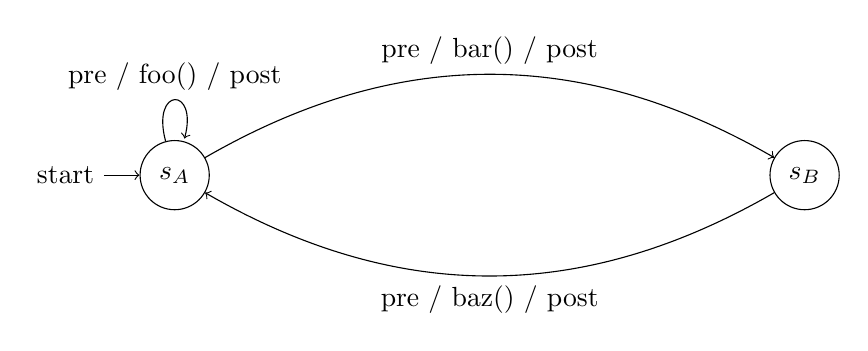
\begin{tikzpicture}[->, auto, node distance=8cm]
      \node[initial,state] (A)              {$s_{A}$};
      \node[state]         (B) [right of=A] {$s_{B}$};

      \path (A) edge [loop above] node {pre / foo() / post} (A)
                edge [bend left]  node {pre / bar() / post} (B)
            (B) edge [bend left]  node {pre / baz() / post} (A);
    \end{tikzpicture}
  \end{center}
\end{frame}

%%%%% 4 Minutes (25)

\section{Conclusions}
\label{sec:conc}

\begin{frame}{Combined approaches}
  % PAPERS: statver, unified

  \only<1,3>{
    Static analysis and runtime verification give different
    viewpoints.

    \vspace{0.25cm}

    \visible<3>{
      Work has been done on:

      \begin{itemize}
        \item Static verification of dynamically-detected
          invariants \parencite{statver},

        \item Using static verification to simplify or even eliminate
          monitoring obligations \parencite{unified}.
      \end{itemize}
    }
  }

  \only<2>{
    \begin{center}
      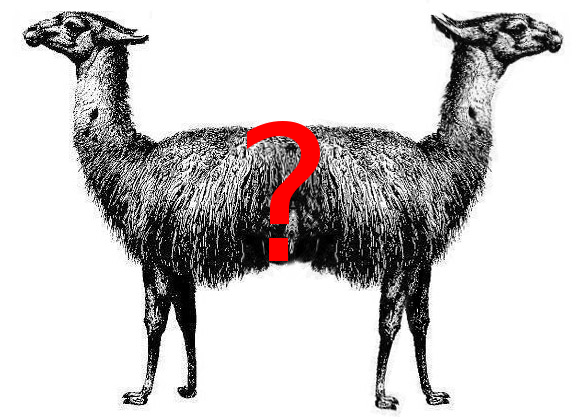
\includegraphics[width=0.75\textwidth]{pushmi-pullyu.png}
    \end{center}
  }
\end{frame}

\begin{frame}{Successes}
  % PAPERS: valgrind, compensate, datarace, addrsan

  \begin{itemize}
    \item Valgrind \parencite{valgrind}
    \item AddressSanitizer: A Fast Address Sanity
      Checker \parencite{addrsan}.
    \item Dynamic Race Detection with LLVM
      Compiler \parencite{datarace}.
    \item Asynchronous monitoring with the ability to roll
      back incomplete transactions \parencite{compensate}.
  \end{itemize}
\end{frame}

\begin{frame}{Open Problems}
  
\end{frame}

\begin{frame}{Runtime Verification: \small A Summary}
  \begin{itemize}
    \item<1-> Only reasons about the current execution
    \item<1-> ``More decidable'' than static analysis
    \item<2-> But not incompatible with static analysis!
    \item<3-> Still a lot to be done in efficient and safe monitoring
      / error recovery
  \end{itemize}
\end{frame}

\begin{frame}{Questions?}
  \vspace{4.5cm}

  \footnotesize
  \textbf{Q:} What is the two-headed creature a few slides back?\\
  \textbf{A:} A pushmi-pullyu, from \textit{The Story of Doctor Dolittle}.

  \begin{quote}
    ``I notice,'' said the duck, ``that you only talk with one of your
    mouths. Can't the other head talk as well?''

    ``Oh, yes,'' said the pushmi-pullyu. ``But I keep the other mouth
    for eating---mostly. In that way I can talk while I am eating
    without being rude. Our people have always been very polite.''
  \end{quote}
\end{frame}

\end{document}